\chapter*{2020年\textsf{HDU}「大学物理1」期中试题解答}

\begin{minipage}{0.32\textwidth}
    \textbf{开课学院}：理学院
      
    \textbf{课程编码}：A0715011
\end{minipage}
\hfill
\begin{minipage}{0.32\textwidth}
    \textbf{解析制作}：\textsf{M.Xia@WeYoung}

    \textbf{\,\hologo{TeX}~排版}：\textsf{M.Xia}
\end{minipage}
\hfill
\begin{minipage}{0.15\textwidth}
    \centering
    \begin{tikzpicture}
        \node [inner sep=0] at (0,0) {
            \qrcode[height=3em,version=4]{https://qm.qq.com/q/mgD30uPiSs}};
        \fill [color=white,rounded corners=(sqrt(2)+2)/11*1em] (-.5em,-.5em) rectangle (.5em,.5em);
        \node [inner sep=0] at (0,0) {\color{MidnightBlue}\scriptsize\faIcon{qq}};
    \end{tikzpicture}

    \scriptsize\href{https://qm.qq.com/q/mgD30uPiSs}{\itshape 未央物理营}
\end{minipage}
\hfill
\begin{minipage}{0.15\textwidth}
    \centering
    \begin{tikzpicture}
        \node [inner sep=0] at (0,0) {
            \qrcode[height=3em,version=4]{http://weixin.qq.com/r/DBIABcHEqgnWKIVmb0eI}};
            \fill [color=white,rounded corners=(sqrt(2)+2)/11*1em] (-.5em,-.5em) rectangle (.5em,.5em);
        \node [inner sep=0] at (0,0) {\color{DarkGreen}\scriptsize\faIcon{weixin}};
    \end{tikzpicture}

    \scriptsize\href{http://weixin.qq.com/r/DBIABcHEqgnWKIVmb0eI}{\itshape 未央学社}
\end{minipage}

\section{选择题（每题3分，共30分）}

\begin{problem}
    根据瞬时速度矢量$\bm v$的定义，在直角坐标系下，其大小$\abs{\bm v}$可表示为
    \begin{tasks}(2)
        \task $\displaystyle\odv rt$
        \task $\displaystyle\abs{\odv xt\bm i}+\abs{\odv yt\bm j}+\abs{\odv zt\bm k}$
        \task[\true] $\displaystyle\sqrt{\ab(\odv xt)^2+\ab(\odv yt)^2+\ab(\odv zt)^2}$
        \task $\displaystyle\odv xt+\odv yt+\odv zt$
    \end{tasks}
\end{problem}
\solute3
\begin{solution}
    直角坐标下速度的大小即其三个方向分量的平方和的算数平方根.
\end{solution}

\begin{problem}
    在地面静止的坐标系内，$A$船以速率$v_1$沿$x$轴正向匀速行驶，$B$船以速率$v_2$沿$y$轴正向匀速行驶，现在$A$船上建立与地面坐标系方向相同的坐标系，则在$A$船中看$B$船的速度为
    \begin{tasks}(4)
        \task $v_1\bm i+v_2\bm j$
        \task[\true] $-v_1\bm i+v_2\bm j$
        \task $-v_1\bm i-v_2\bm j$
        \task $v_1\bm i-v_2\bm j$
    \end{tasks}
\end{problem}
\solute3
\begin{solution}
    由相对运动关系得$\bm v_{BA}=\bm v_B-\bm v_A=v_2\bm j-v_1\bm i$.
\end{solution}

\begin{problem}
    \begin{paracol}{2}
    如图所示，一匀质细杆可绕通过左端与杆垂直的水平光滑固定轴O旋转，初始状态为静止悬挂. 现有一个小球自左方水平打击细杆. 设小球与细杆之间为非弹性碰撞，则在碰撞过程中对细杆与小球这一系统
    \switchcolumn\vspace*{\fill}\centering
    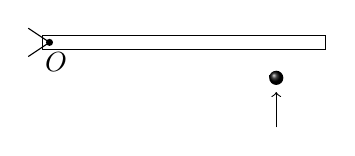
\begin{tikzpicture}[scale=.9,rotate=90]
        \wall{(-1,0)}{(1,.1)};
        \draw (-.1,-4.2) rectangle + (.2,4);
        \draw (-.2,0) -- (0,-.3) -- (.2,0);
        \fill (0,-.3) circle (.05);
        \shade [ball color=black] (-.5,-3.5) circle (.1);
        \draw [->] (-1.2,-3.5) -- (-.7,-3.5);
        \node [anchor=north west] at (0,-.1) {$O$};
    \end{tikzpicture}
    \vspace*{\fill}
    \end{paracol}
    \begin{tasks}(2)
        \task 只有机械能守恒
        \task 只有动量守恒
        \task[\true] 只有对转轴$O$的角动量守恒
        \task 机械能、动量和角动量均守恒
    \end{tasks}
\end{problem}
\solute2
\begin{solution}
    由于小球与细杆之间为非弹性碰撞，所以二者机械能不守恒；碰撞时，转轴对杆的作用力有水平方向分量，所以动量不守恒；转轴处的作用力对转轴力矩为零，所以角动量守恒.
\end{solution}

\begin{problem}
    一长$l$，质量$m$的船浮于静水中，一个质量也为$m$的人从船尾走到船头. 不计水和空气的阻力，则在此过程中船将
    \begin{tasks}(4)
        \task 不动
        \task 后退$l$
        \task[\true] 后退$l/2$
        \task 后退$l/3$
    \end{tasks}
\end{problem}
\solute4
\begin{solution}
    人船系统水平方向上动量守恒，质心位置不变. 设人在行走过程中船运动的距离为$x$，由于二者的位置变化对系统质心位置变化的贡献为零，所以有
    \[m(l+x)+mx=0\]
    其中$l+x$为人相对地面的位移. 解得$x=-l/2$，负号表示船与人的运动方向相反，即后退$l/2$.
\end{solution}

\begin{paracol}{2}
\begin{problem}
    如图所示，将一根轻绳绕绕过一滑轮边缘，绳与滑轮之间无滑动，若分别将质量为$m$的砝 码挂在绳端和用恒力为$F=mg$向下拉绳端. 分别用$\beta_a$和$\beta_b$表示两种情况下滑轮的角加速度，则
    \begin{tasks}(4)
        \task $\beta_a>\beta_b$
        \task $\beta_a=\beta_b$
        \task[\true] $\beta_a<\beta_b$
        \task 不确定
    \end{tasks}
    \switchcolumn\vspace*{\fill}\centering
    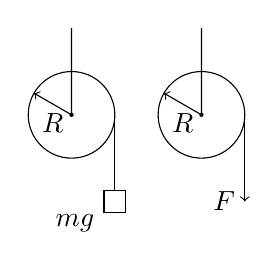
\begin{tikzpicture}[scale=.55]
        \wall{(-1,0)}{(1,.2)};
        \draw (0,0) -- (0,-2) circle (1);
        \fill (0,-2) circle (.05);
        \draw (1,-2) -- (1,-3.75) (.75,-4.25) rectangle + (.5,.5);
        \node [left] at (.75,-4.5) {$mg$};
        \draw [->] (0,-2) -- ({-sqrt(3)/2},-1.5) node [midway,below] {$R$};

        \wall{(2,0)}{(4,.2)};
        \draw (3,0) -- (3,-2) circle (1);
        \fill (3,-2) circle (.05);
        \draw [->] (4,-2) -- (4,-4) node [left] {$F$};
        \draw [xshift=3cm,->] (0,-2) -- ({-sqrt(3)/2},-1.5) node [midway,below] {$R$};
    \end{tikzpicture}\vspace*{\fill}
\end{problem}
\end{paracol}
\solute1
\begin{note}\leavevmode
\begin{itemize}
    \item 下落过程中物体也要增加自己的动能，所以会``拖累''滑轮的加速转动过程. 所以直接用拉力$P$去拉绳子使滑轮获得的角加速度要比重物带着绳子使滑轮获得的角加速度大.
    \item 重物加速下落的过程中属于失重过程，绳子的拉力一定小于其重力$P$，进而拉力对滑轮的力矩就小于$PR$，所以前者角加速度要比后者小，即直接用拉力$P$去拉绳子使滑轮获得的角加速度要比重物带着绳子使滑轮获得的角加速度大.
\end{itemize}
\end{note}
\begin{solution}
    设绳子拉力为$T$. 对重物列牛顿运动定律、对滑轮列转动定律得
    \[\begin{dcases}
        mg-T=ma\\
        TR=I\beta_a
    \end{dcases}\]
    由线量和角量之间的关系$a=R\beta_a$联立以上两式得$\beta_a=mgR/(mR^2+I)<mgR/I=\beta_b$.
\end{solution}

\begin{problem}
    轮圈半径为$R$，其质量M均匀布在轮缘上，长为$R$，质量为m的均质辐条固定在轮心和轮缘间，辐条共有$2N$根. 今若将辐条数减少$N$根但保持轮对通过轮心，垂直于轮平面轴的转动惯量保持不变，则轮圈的质量为
    \begin{tasks}(4)
        \task $Nm/12+M$
        \task $Nm/6+M$
        \task $2Nm/3+M$
        \task[\true] $Nm/3+M$
    \end{tasks}
\end{problem}
\solute1
\begin{solution}
    由总体转动惯量保持不变得$MR^2+2N\cdot\frac{1}{3}ml^2=M'R^2+N\cdot\frac{1}{3}ml^2$，解得后来轮圈的质量为$M'=M+Nm/3$.
\end{solution}

\begin{paracol}{2}
\begin{problem}
    如图所示，在原点放一正电荷Q，它在P点$(x=+1,y=0)$产生的电场强度为$\bm E$. 现在，另外有一个负电荷$-2Q$，试问应将它放在何处才能使$P$点的电场强度等于零
    \begin{tasks}(3)
        \task $x$轴$x>1$
        \task $x$轴$0<x<1$
        \task[\true] $x$轴$x<0$
        \task $y$轴$y>0$
        \task $y$轴$y<0$
    \end{tasks}
    \switchcolumn\vspace*{\fill}\centering
    \begin{tikzpicture}[scale=.9]
        \draw [->] (-1,0) -- (3,0) node [below] {$x$};
        \draw [->] (0,-1) -- (0,2) node [left] {$y$};
        \shade [ball color=MidnightBlue] (0,0) circle (.1) node [below right] {$O$} node [above left] {$+Q$};
        \fill (1.5,0) circle (.05) node [below] {$P$} node [above] {$(1,0)$};
    \end{tikzpicture}\vspace*{\fill}
\end{problem}
\end{paracol}
\solute0
\begin{solution}
    $+Q$在$P$点场强方向水平向右，需要$-2Q$在$P$点产生一个水平向左的场强进行抵消，所以$-2Q$一定在$x$轴上$P$点左侧. 又因为其电量比$Q$大，所以其与$P$的距离比$Q$与$P$的距离大，所以其在$x$轴负半轴.
\end{solution}

\begin{paracol}{2}
\begin{problem} % {动量定理}
    如图所示，质量为$m$的质点，沿正三角形$ABC$的水平光滑轨道匀速度$\bm v$运动，质点越过$A$点时，轨道作用于质点的冲量的大小
    \begin{tasks}(4)
        \task $mv$
        \task $\sqrt{2}mv$
        \task $\sqrt{3}mv$
        \task $2mv$
    \end{tasks}
\end{problem}
\switchcolumn\vspace*{\fill}\centering
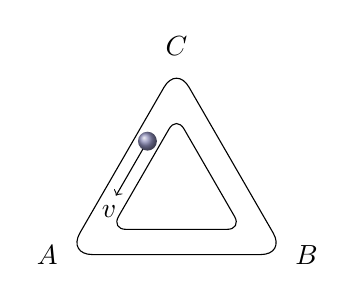
\begin{tikzpicture}[scale=.8]
    \draw [rounded corners=9] (0,2) node [above] {$C$} -- ({-sqrt(3)},-1) node [left] {$A$} -- ({sqrt(3)},-1) node [right] {$B$} -- cycle;
    \draw [scale=.6,rounded corners=5.4] (0,2) -- ({-sqrt(3)},-1) -- ({sqrt(3)},-1) -- cycle;
    \draw [->] ({-.8/sqrt(3)},.8) --++ (-.5,{-.5*sqrt(3)}) node [below,xshift=-sin(30)*.5em,] {$\bm v$};
    \shade [ball color=MidnightBlue!50] ({-.8/sqrt(3)},.8) circle (.15);
\end{tikzpicture}\vspace*{\fill}
\switchcolumn
\solute0
\begin{solution}
    $\abs{\Delta\bm p}=\abs{mv\bm i-\ab(-\frac12mv\bm i-\frac{\sqrt3}2mv\bm j)}=\sqrt3mv$.
\end{solution}
\end{paracol}

\begin{paracol}{2}
\begin{problem}
    空间有一非均匀电场，其电场线如图所示. 若在电场中取一半径为$R$的球面，已知通过球面上$\Delta S$面的电通量为$\Delta\Phi_e$，则通过其余部分球面的电通量为
    \begin{tasks}(2)
        \task[\true] $-\Delta\Phi_e$
        \task $4\pi R^2\Delta\Phi_e/\Delta S$
        \task $(4\pi R^2-\Delta S)\Delta\Phi_e/\Delta S$
        \task $0$
    \end{tasks}
\end{problem}
\switchcolumn\vspace*{\fill}\centering
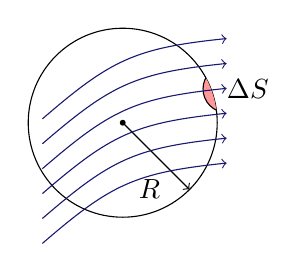
\begin{tikzpicture}[scale=.6]
    \filldraw [draw] (0,0) circle (.05);
    \begin{scope}
    \clip [draw] (0,0) circle (2);
    \filldraw [red!40,draw=black] (2.2,.715) circle  (.5);
    \end{scope}
    \node [anchor=west] at (2,.715) {$\Delta S$};
    \draw [->] (0,0) -- (1.414,-1.414);
    \node [anchor=north east] at (1,-1) {$R$};
    \foreach \i in {-30, -15, 0, 15, 30, 45}
    \draw [->,MidnightBlue,yshift=\i] (-1.7,-1.5) .. controls (-.25,-.25) and (.25,0) .. (2.2,.2);
\end{tikzpicture}\vspace*{\fill}
\end{paracol}
\solute0
\begin{solution}
    由于球面内没有电荷，所以从球面进入的电通量=从球面出来的电通量，球面净电通量为零. 则若已知通过球面上$\Delta S$面的电通量为$\Delta\Phi_e$，那么通过其余部分球面的电通量为$-\Delta\Phi_e$.
\end{solution}

\begin{problem}
    一个带电的绝缘体靠近一个不带电的导体球，则在绝缘体和导体球之间
    \begin{tasks}(6)
        \task*(2) 不存在电力
        \task*(2) 存在相互排斥力
        \task*(2)[\true] 存在相互吸引力
        \task! 吸引力还是排斥力取决于绝缘体带正电还是带负电
    \end{tasks}
\end{problem}
\begin{solution}
    无论绝缘体带正电还是负电，其都会使导体球下表面产生与其电性相反的感应电荷. 虽然导体球需保证总电量为零而在上表面产生与其电量相同的电荷，但是上表面的电荷与绝缘体的距离比下表面的电荷与绝缘体的距离远，所以最终结果还是由下表面主宰，二者始终存在吸引力.
\end{solution}

\section{填空题（共20分）}

\begin{problem}
    将一负电荷从无穷远处移到一个不带电的导体附近，则导体内的电场强度\ans{不变}；导体的电势\ans{减小}（填增大、不变、减小）.
\end{problem}
\begin{solution}
    静电平衡时，导体内部没有场强，故其电场强度不变；由于该电荷带负电，故当电荷靠近时，导体的电势减小.
\end{solution}

\begin{paracol}{2}
\begin{problem}
    电荷$q_1$，$q_2$，$q_3$和$q_4$在真空中的分布如图所示，其中$q_2$是半径为$R$的均匀带电球体，$S$为闭合曲面，则通过闭合曲面$S$的电通量$\oint_S{\bm E\cdot\d\bm S}=$\ans{$(q_1+q_2)/\epsilon_0$}.
    \switchcolumn\vspace*{\fill}\centering
    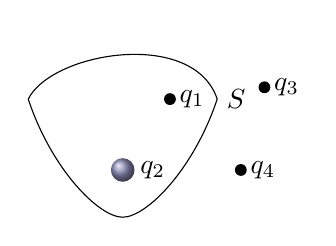
\begin{tikzpicture}[scale=1.5]
        \draw(-.8,.4) .. controls (-.6,.8) and (.6,1) .. (.8,.4) node [right] {$S$} .. controls (.6,-.2) and (.2,-.6) .. (0,-.6) .. controls (-.2,-.6) and (-.6,-.2) .. (-.8,.4);
        \fill (.4,.4) circle (.05) node [right] {$q_1$};
        \shade [ball color=MidnightBlue!50] (0,-.2) circle (.1) node [right,xshift=.1cm] {$q_2$};
        \fill (1.2,.5) circle (.05) node [right] {$q_3$};
        \fill (1,-.2) circle (.05) node [right] {$q_4$};
    \end{tikzpicture}\vspace*{\fill}
\end{problem}\switchcolumn
\solute0
\begin{solution}
    由高斯定理，通过闭合曲面的电通量只与其内部所包电荷，即$q_1$，$q_2$有关. 故$\Phi_e=(q_1+q_2)/\epsilon_0$.
\end{solution}
\end{paracol}

\begin{problem}
    真空中电量分别为$q_1$，$q_2$的两个点电荷，当它们相距为$r$时，该电荷系统的相互作用电势能$W=$\ans{$q_1q_2/4\pi\epsilon_0r$}（设当两个点电荷相距无穷远时电势能为零）.
\end{problem}
\begin{solution}
    $W_{12}=(q_1V_{21}+q_2V_{12})/2=(q_1q_2/4\pi\epsilon_0r+q_2q_1/4\pi\epsilon_0r)/2=q_1q_2/4\pi\epsilon_0r$.
\end{solution}

\begin{problem}
    在一个转动的齿轮上，一个齿尖$P$做半径为$R$的圆周运动，其路程$s$随时间的变化规律为$s=v_0t+bt^2/2$，其中$v$和$b$都是正的常量，则$t$时刻，齿尖$P$的速度大小$v=$\ans{$v_0+bt$}，加速度大小$a=$\ans{$\sqrt{(v_0+bt)^4/R^2+b^2}$}.
\end{problem}
\solute0
\begin{solution}
    路程对时间求导得速度大小$v=\odv st=v_0+bt$，再求导得切向加速度大小$a_\tau=\odv vt=b$，法向加速度大小$a_n=v^2/R=(v_0+bt)^2/R$，加速度大小$a=\sqrt{a_\tau^2+a_n^2}=\sqrt{(v_0+bt)^4/R^2+b^2}$.
\end{solution}

\begin{paracol}{2}
\begin{problem}
    质量为$m$的小球，以水平速度$\bm v_1$与光滑桌面上质量为$M$的静止斜劈作完全弹性碰撞后竖直弹起，如图所示，则碰后斜劈的运动速度值\ans{$mv_1/M$}.
    \switchcolumn\vspace*{\fill}\centering
    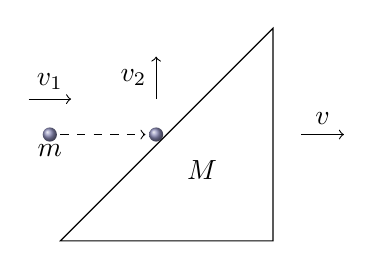
\begin{tikzpicture}[scale=.9]
        \wall{(-.5,0)}{(4.5,-.2)};
        \draw (0,0) -- (3,0) -- (3,3) -- cycle;
        \node at (2,1) {$M$};
        \draw [dashed,->] (0,1.5) -- (1.2,1.5);
        \shade[ball color=MidnightBlue!50] (-.15,1.5) circle (.1) node [below] {$m$};
        \shade[ball color=MidnightBlue!50] (1.35,1.5) circle (.1);
        \draw [->] (-.45,2) -- (.15,2) node [midway,above] {$v_1$};
        \draw [->] (1.35,2) -- (1.35,2.6) node [midway,left] {$v_2$};
        \draw [->] (3.4,1.5) -- (4,1.5) node [midway,above] {$v$};
    \end{tikzpicture}\vspace*{\fill}
\end{problem}\switchcolumn
\solute0
\begin{solution}
    小球与斜劈在水平方向上动量守恒$mv_1+0=0+Mv$，得碰后斜劈的运动速度大小为$v=mv_1/M$.
\end{solution}
\end{paracol}

\begin{problem}
    转动着的飞轮的转动惯量为$I$，在$t=0$时角速度为$\omega_0$. 此后飞轮经历制动过程，阻力矩$M$的大小与角速度$\omega$的平方成正比，比例系数为$k$（$k>0$）. 当$\omega=\omega_0/3$时，飞轮的角加速度\ans{$-k\omega_0^2/9I$}.
\end{problem}
\solute0
\begin{solution}
    由转动定律$-k\omega^2=I\beta$，当$\omega=\omega_0/3$时，角加速度为$\beta=-k\omega_0^2/9I$.
\end{solution}

\begin{problem}
    平行板电容器充电结束时，极板带电为$Q_0$，极板之间的电场强度大小为$E_0$. 现保持电源连接，使两极板间充满相对介电常数为$\epsilon_r$的各向同性均匀电介质，这时极板上的电量$Q=$\ans{$\epsilon_rQ_0$}，极板间电场强度$E=$\ans{$E$}.
\end{problem}
\solute0
\begin{solution}
    平行板带电量为$Q=UC$. 由于电容器保持电源连接，所以极板间电场强度不变，极板间电压不变. 由于平行板电容器电容表达式为$C=\epsilon_r\epsilon_0S/d$，所以极板上的电量$Q\propto C$. 而充满电介质后，$C'=\epsilon_rC$，故$Q=\epsilon_rQ_0$.
\end{solution}

\clearpage
\section{计算题（每题10分，共50分）}

\begin{paracol}{2}
\begin{problem}
    如图所示，两个大小不同、具有水平光滑轴的定滑轮，定点在同一水平线上. 小滑轮的质量为$m$，半径$r$，对轴的转动惯量$I=mr^2/2$，大滑轮的质量$m'=2m$、半径$r'=2r$，对轴的转动惯量$I'=m'r'^2/2$. 一根不可伸缩的轻质细绳跨过两个定滑轮，绳的两端分别挂着物体$A$和$B$. $A$的质量为$m$，$B$的质量为$m'=2m$. 这一系统由静止开始转动. 求两滑轮的角加速度和它们之间绳子的张力.
    \switchcolumn\vspace*{\fill}\centering
    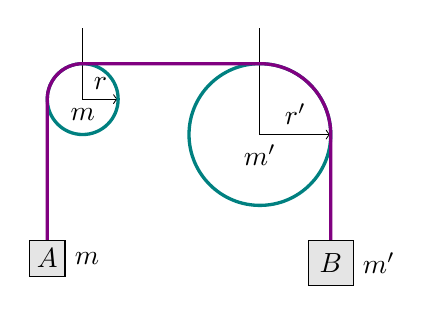
\begin{tikzpicture}[scale=.9]
        \wall{(-1.2,1)}{(4.2,1.2)};
        \draw [->] (0,1) -- (0,0) node [below] {$m$} -- (.5,0) node [midway,above] {$r$};
        \draw [very thick,teal] (0,0) circle (.5);
        \draw [->] (2.5,1) -- (2.5,-.5) node [below] {$m'$} -- (3.5,-.5) node [midway,above] {$r'$};
        \draw [very thick,teal] (2.5,-.5) circle (1);
        \draw [very thick,color=violet] (-.5,-2) -- (-.5,0) arc (180:90:.5) -- (2.5,.5) arc (90:0:1) -- (3.5,-2);
        \filldraw [gray!20,draw=black] (-.75,-2) rectangle (-.25,-2.5) node [black,midway] {$A$} node [black,right] at (-.25,-2.25) {$m$};
        \filldraw [gray!20,draw=black] ({3.5-.5*2^(1/3)/2},-2) rectangle + ({.5*2^(1/3)},{-.5*2^(1/3)}) node [black,midway] {$B$} node [black,right] at ({3.5+.5*2^(1/3)/2},{-2-.5*2^(1/3)/2}) {$m'$};
    \end{tikzpicture}\vspace*{\fill}
\end{problem}
\end{paracol}
\solute{-2}
\begin{multicols}{2}
\begin{solution}
    设二者之间绳子的张力为$T$，悬挂$A$、$B$绳子的张力分别为$T_A$、$T_B$. 对$A$，$B$和两个滑轮，分别由牛顿运动定律和转动定律得
    \[\begin{dcases}
        T_A-mg=ma\\
        m'g-T_B=m'a\\
        Tr-T_Ar=I\beta_1\\
        T_Br'-Tr'=I'\beta_2
    \end{dcases}\]
    利用关系$\beta_1r=\beta_2r'=a$联立以上五式得
    \begin{itemize}
        \item $\displaystyle\beta_1=\frac{(m'-m)g}{(m+m')r+I/r+I'r/r'^2}$
        \item $\displaystyle\beta_2=\frac{(m'-m)g}{(m+m')r'+Ir'/r^2+I'/r'}$
        \item $\displaystyle a=\frac{(m'-m)g}{m+m'+I/r^2+I'/r'^2}$
        \item $T=ma+mg+Ia/r^2$
    \end{itemize}
\end{solution}
\end{multicols}

\begin{paracol}{2}
\begin{problem}
    如图所示，质量为$m$的子弹以速度$\bm v_0$水平射入沙土中，如果子弹受到的阻力与速度大小成正比，比例系数为$k$，忽略子弹的重力.求
    \begin{enumerate}
        \item 子弹射入沙土后的速度随时间变化关系.
        \item 子弹进入沙土的最大深度.
    \end{enumerate}
    \switchcolumn\vspace*{\fill}\centering
    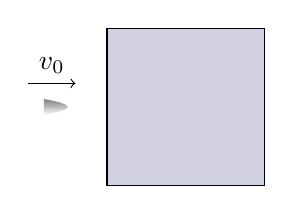
\begin{tikzpicture}
        \filldraw [fill=MidnightBlue!20] (-1,1) rectangle (1,-1);
        \shade [rotate=-90] (-.1,-1.8) parabola bend (0,-1.5) (.1,-1.8)--cycle;
        \draw [->] (-2.0,.3) -- (-1.4,.3) node [above,midway] {$\bm v_0$};
    \end{tikzpicture}\vspace*{\fill}
\end{problem}    
\end{paracol}
\solute1
\begin{solution}\leavevmode
    \begin{enumerate}
        \item 子弹加速度$a=-kv/m=\d v/\d t$，分离变量并积分得速度表达式$v=v_0\e^{-kt/m}$.
        \item 对速度积分得$x=mv_0(1-\e^{-kt/m})/k$. 当$t\to\infty$时，子弹达到最深处，$x=x_{\max}=mv_0/k$.
    \end{enumerate}
\end{solution}

\begin{problem}
    电荷以相同的面密度$\sigma$分布在$r_1=\qty{10}\cm$和$r_2=\qty{20}\cm$的两个同心球面上，设无限远处的电势为零，球心处的电势为$\varphi=\qty{300}\V$. 求
    \begin{enumerate}
        \item 电荷面密度$\sigma$.
        \item 如果使球心处的电势为零，外球面上应放掉多少电荷?
    \end{enumerate}
\end{problem}
\solute1
\begin{solution}\leavevmode
    \begin{enumerate}
        \item 球心处电势$\displaystyle\varphi=\sigma\cdot 4\pi r_1^2/4\pi\epsilon_0r_1+\sigma\cdot 4\pi r_2^2/4\pi\epsilon_0r_2=\qty{300}\V$，解得$\sigma=\qty{8.85e-9}{\C\cdot\m^{-2}}$.
        \item 由题意，放掉的电荷量对电势的贡献为$\qty{300}\V$，即$\Delta q/4\pi\epsilon_0r_2=\qty{300}\V$. 得$\Delta q=\qty{6.67e-9}\C$.
    \end{enumerate}
\end{solution}

\begin{paracol}{2}
\begin{problem}
    如图所示，长为$l$、质量为$m_1$的均匀细杆可绕端点$O$固定水平光滑轴转动. 杆从水平位置以初角速度$\omega_0$释放，摆到竖直位置时和光滑水平桌面上的小球相碰. 球的质量为$m_2$. 设碰撞是弹性碰撞，求碰后小球获得的速度.
    \switchcolumn\vspace*{\fill}\centering
    \begin{tikzpicture}[scale=.8]
        \wall{(-1,0)}{(1,.15)};
        \draw (-.1,-4.2) rectangle + (.2,4);
        \draw [dashed] (-.1,-.4) rectangle + (4,.2);
        \draw [rounded corners=2pt] (-.2,0) -- (0,-.3) -- (.2,0);
        \fill (0,-.3) circle (.05);
        \shade[ball color=MidnightBlue!50] (-.3,-4) circle (.2);
        \draw [<-] (-1.2,-4) -- (-.7,-4);
        \node [anchor=north east] at (0,-.1) {$O$};
        \node [anchor=south] at (-.95,-4) {$\bm v$};
        \node [anchor=south] at (-.3,-3.8) {$\scriptstyle m_2$};
        \node [anchor=north] at (2.1,-.4) {$\scriptstyle m_1$};
        \draw [yshift=-.3cm,->] ({cos(30)},{-sin(30)}) arc (-30:-60:1) node [below] {$\omega$};
        \wall{(-1.5,-4.22)}{(1.5,-4.42)};
    \end{tikzpicture}\vspace*{\fill}
\end{problem}\switchcolumn
\solute2
\begin{solution}
    细杆从释放到与小球碰撞前，由动能定理
    \[m_1g\frac l2=\frac12I\omega^2-\frac12I\omega_0^2\]
\switchcolumn*[\noindent %
    其中$I=m_1l^2/3$为细杆绕转轴的转动惯量. 得碰撞前细杆的角速度为
    \[\omega=\sqrt{\omega_0^2+\frac{m_1gl}{I}}\]
    分别由碰撞时细杆和小球对转轴角动量守恒、机械能守恒得
    \[\begin{cases}
        I\omega=m_2vl+I\omega'\\
        \displaystyle\frac12I\omega^2=\frac12I\omega'^2+\frac12m_2v^2
    \end{cases}\]
    解得碰后小球获得的速度为$v=2m_1\sqrt{\omega_0^2l^2+3gl}/(m_1+3m_2)$.]
\end{solution}
\end{paracol}

\begin{problem}
    用绝缘细线弯成的半圆环，半径为$R$，其上均匀地带有正电荷$Q$，试求圆心$O$点的电场强度.
\end{problem}
\solute1
\begin{solution}
    如图所示，作圆环上任一线元$\d l$到$O$点连线的反向延长线，与圆环顶端的切线相交于$A$，$B$两点. 由图中几何关系得，$AB=r'\d\theta/\sin\theta=R\d\theta/\sin^2{\theta}$.
        
    \begin{figure}[htbp]
        \centering
        \begin{tikzpicture}
            \draw [very thick,dashed] (-3,2) node [above] {$M$} -- (3,2) node (n) [above] {$N$};
            \draw [very thick] (-2.5,2) -- (2.5,2);
            \draw (-2,0) arc (180:0:2);
            \draw [->] (0,0) node [right] {$O$} -- (0,2) node [right,midway] {$R$};
            \draw [very thick,teal] (-2.5,2) node [above,black] {$\scriptstyle A$} -- (-2,2) coordinate (b) node [above,black] {$\scriptstyle B$} -- (0,0) -- cycle;
            \filldraw (0,0) coordinate (o) circle (.05);
            \pic["$\theta$", draw=DarkRed,very thick,angle eccentricity=1.5,angle radius=12]{angle=o--b--n};
            \draw [dotted] (b) -- ({-10*sqrt(82)/41},{8*sqrt(82)/41}) coordinate (d) node [below left] {$\scriptstyle D$};
            \draw [decorate,decoration={brace,raise=2pt}] (o) -- (d) node [midway,below left] {$r'$};
        \end{tikzpicture}
    \end{figure}
    而圆环上线元在$O$点产生的场强大小为$\d E=\lambda\d\theta/4\pi\epsilon_0R$.
    若顶端的切线均匀带电，电荷线密度为$\lambda'$，则$AB$在$O$点产生的场强大小为
    \[\d E'=\frac{1}{4\pi\epsilon_0}\frac{\lambda'AB}{r'^2}=\frac{1}{4\pi\epsilon_0}\frac{\lambda'R\d\theta/\sin^2{\theta}}{(R/\sin\theta)^2}
    =\frac{1}{4\pi\epsilon_0}\frac{\lambda'\d\theta}{R}\]
    若$\lambda'=\lambda$，则$\d E'=\d E$. 意味着均匀带电半圆环可由带有等量电荷线密度的无限长直线替代. 由高斯定理，无限长直带电线在距其$R$处的场强大小为$E=\lambda/2\pi\epsilon_0R\xlongequal{\lambda=Q/\pi R}Q/2\pi^2\epsilon_0R^2$.
\end{solution}